\documentclass[tikz]{standalone}
\usepackage{amsmath}
\usepackage{xcolor}
\usetikzlibrary{calc,arrows.meta}
\definecolor{bg}{HTML}{171D2B}
\definecolor{acc}{HTML}{F7B538}
\begin{document}
\pagecolor{bg}
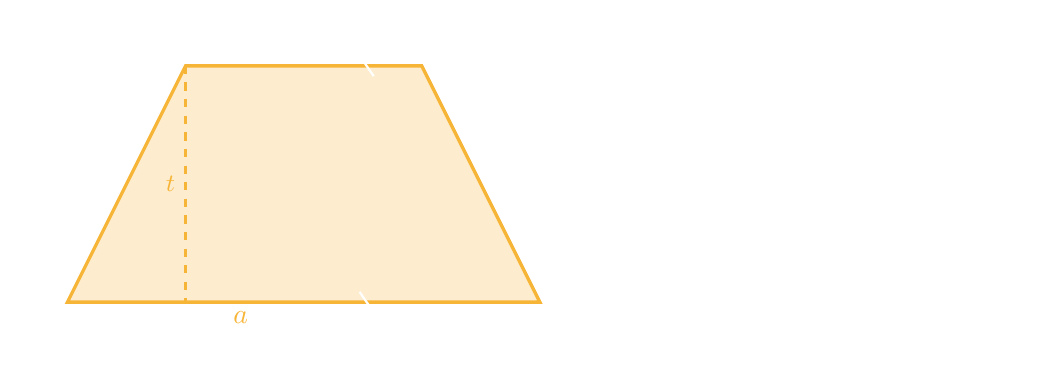
\begin{tikzpicture}[scale=1.0]
\coordinate (A) at (0,0);
\coordinate (B) at (6,0);
\coordinate (C) at (4.5,3);
\coordinate (D) at (1.5,3);
% salinan diputar 180 derajat digambar dulu (di belakang)
\begin{scope}[rotate around={180:(3,1.5)}]
  \draw[very thick, draw=white!70, fill=white!10] (A) -- (B) -- (C) -- (D) -- cycle;
\end{scope}
% trapesium asli di depan
\draw[very thick, draw=acc, fill=acc!25] (A) -- (B) -- (C) -- (D) -- cycle;
\path (A) node[below left, white] {$A$} (B) node[below right, white] {$B$}
      (C) node[above right, white] {$C$} (D) node[above left, white] {$D$};
% tanda sama kaki (geser dari tengah agar tidak menimpa label)
\draw[thick, white] ($(A)!0.5!(B)+(0.8,0)$) ++(-0.09,0.13) -- ++(0.18,-0.26);
\draw[thick, white] ($(D)!0.5!(C)+(0.8,0)$) ++(-0.09,0.13) -- ++(0.18,-0.26);
% tinggi dan alas
\draw[dashed, thick, acc] (1.5,3) -- (1.5,0) node[midway, left, acc, font=\small] {$t$};
\node[below, acc] at (2.2,0) {$a$};
\node[above, white] at (2.2,3) {$b$};
\draw[-{Latex[length=2mm]}, thick, white] (7.5,1.5) -- (8.7,1.5);
\node[anchor=west, white, font=\small, align=left] at (8.8,1.5)
  {dua trapesium\\disatukan\\menjadi jajargenjang};
\end{tikzpicture}
\end{document}
